\begin{surferPage}{많은 실수 특이점을 가지는 곡면}
    앞서 말했듯이 $7$차식의 최대 특이점 수 $\mu(7)$ 은 알려져 있지 않습니다. 우리가 수학적 증명을 통해 알고 있는 사실은 상한과 하한 뿐입니다:
$99\le \mu(7) \le 104$.


    그러므로 일반적 차수 $d$ 에 대해서 알려진 사실이 거의 없다는 것이 그다지 놀랍지 않습니다. 

    Sonja Breske, Oliver Labs 그리고 Duco van~Straten는 S.V.\ Chmutov 의해 밝혀진 '특이점의 최대 개수는 실수 특이점을 갖는 곡면으로부터 얻어진다' 라는 사실밖에 이용할 수 없었습니다. 다음은 현재까지 밝혀진 성질입니다.
    \[0,41\bar{6}d^3 \lessapprox \mu(d) \lessapprox 0.44\bar{4} d^3.\]
    이로부터 우리는 구조의 대칭성뿐만 아니라 직선의 배열을 통해 얻는 삼각형의 개수와의 관계를 볼 수 있습니다. 

    \begin{center}
      \begin{tabular}{c@{\qquad}c}
        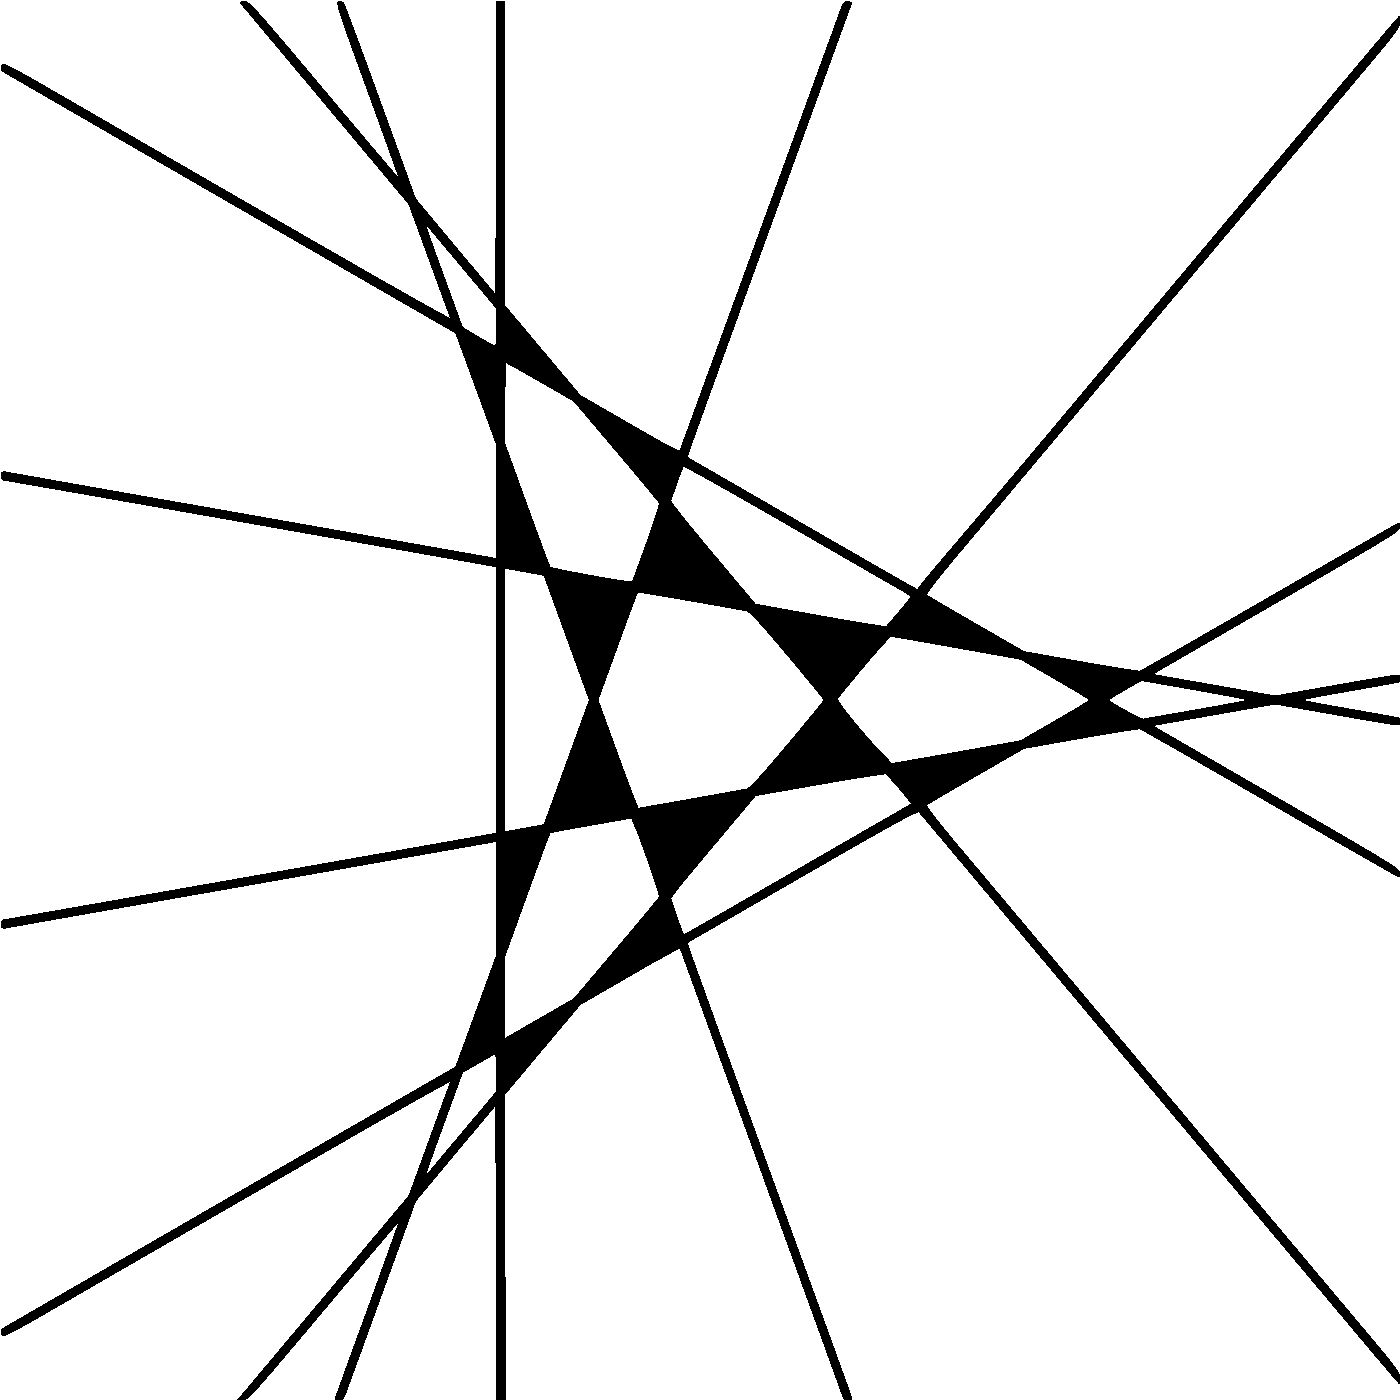
\includegraphics[height=1.5cm]{./../../common/images/vielesing.pdf}
        &
        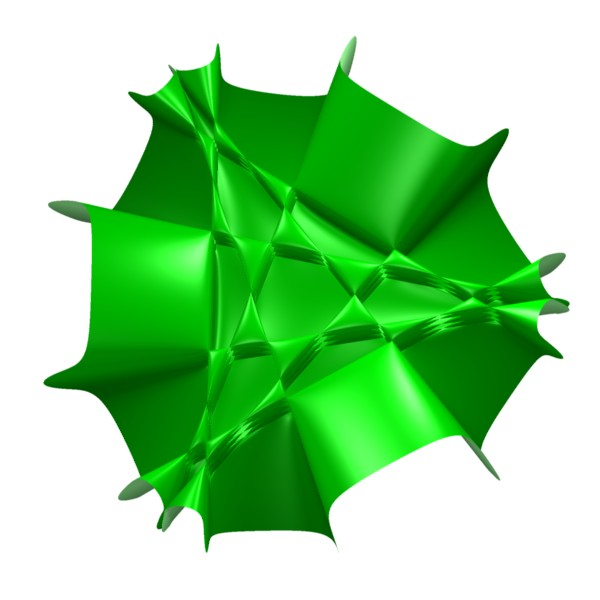
\includegraphics[height=1.5cm]{./../../common/images/p9surface_von_oben}
      \end{tabular}
    \end{center}
\end{surferPage}
